\documentclass[letter,11pt]{article}
%\documentclass[letter,twoside,11pt]{article}

\usepackage[spanish,es-nodecimaldot]{babel}
\usepackage[utf8]{inputenc}

\usepackage{lmodern}
\usepackage[T1]{fontenc}
\usepackage{textcomp}

\usepackage{graphicx}
\usepackage{pstricks}

\usepackage{anysize}
\marginsize{3cm}{2cm}{2cm}{3cm}

\usepackage{amsmath}
\usepackage{array}
\usepackage{gensymb}
\usepackage{alltt}

\usepackage{fancyhdr}
\usepackage{lastpage}
\pagestyle{fancy}
\fancyhf{}
\fancyhead[LE,RO]{Laboratorio de Física Básica I}
\fancyfoot[CO,CE]{\thepage\ de \pageref{LastPage}}

\special{papersize=215.9mm,279.4mm}

\usepackage[
    pdfauthor={Carlos Eduardo Caballero Burgoa},%
    pdftitle={Laboratorio de Física Básica I},%
    pdfsubject={Método de los mínimos cuadrados},%
    colorlinks,%
    citecolor=black,%
    filecolor=black,%
    linkcolor=black,%
    urlcolor=black,
    breaklinks]{hyperref}
\usepackage{breakurl}

\newcommand{\blankpage}{
\newpage
\thispagestyle{empty}
\mbox{}
\newpage
}

\renewcommand{\arraystretch}{1.2}

\begin{document}

\begin{titlepage}
\begin{center}
{\Large UNIVERSIDAD MAYOR DE SAN SIMÓN}\\
\vspace*{0.15cm}
{\large FACULTAD DE CIENCIAS Y TECNOLOGÍA}\\
\vspace*{0.10cm}
DEPARTAMENTO DE FÍSICA\\
\vspace*{3.0cm}
{\Large \textbf{LABORATORIO DE FÍSICA BÁSICA I}}\\
\vspace*{0.3cm}
{\Large \textbf{PRACTICA No. 4}}\\
\vspace*{3.5cm}
{\Large \textbf{MÉTODO DE LOS MÍNIMOS CUADRADOS}}\\
\end{center}

\vspace*{7.4cm}
\leftskip=7.95cm
\noindent
\textbf{Estudiante:}\\
Caballero Burgoa, Carlos Eduardo.\\
\newline
\textbf{Docente:}\\
Msc. Guzmán Saavedra, Rocio.\\
\newline
\textbf{Grupo:} N5.\\
\textbf{Fecha de realización:} 08 de Diciembre del 2020.\\
\textbf{Fecha de entrega:} 11 de Diciembre del 2020.\\

\end{titlepage}

\blankpage

\section{Objetivo}
Desarrollar la destreza de los alumnos en el ajuste de una linea recta por el
método de los mínimos cuadrados.

\section{Marco teórico}
Para obtener la ecuación de la linea recta de los pares de valores $(x,y)$ en
forma analítica, se recurre al método de los mínimos cuadrados.

Considerando el caso de que estos pares de valores se ajustan a una linea recta
y cuando el error de $x$ es pequeño comparado con el error de $y$:

Sea:

\begin{equation}
    Y = A + B X
\end{equation}

Para la ecuación de la mejor linea recta que pasa por los $n$ puntos del
gráfico: $y = f(x)$, se debe cumplir la condición que $\sum {d_i}^2$ sea mínima.

A partir de esta condición podemos determinar los valores de los parámetros $A$
y $B$ de la ecuación para la recta.

Definimos $d_i$ como la discrepancia de las ordenadas, entre los valores
experimentales $y_i$, y los valores obtenidos por la ecuación de la recta $y_i$
para cada uno de los valores de $x_i$.

\begin{equation}
    d_i = y_i - y'_i = y_i - ( A + B x_i )
\end{equation}

Para determinar los valores de $A$ y $B$ derivamos la $\sum {d_i}^2$ respecto de
$A$ y $B$, y obtenemos el siguiente par de ecuaciones:

\begin{equation}
    \sum y_i = A n + B \sum x_i
\end{equation}
\begin{equation}
    \sum x_i y_i = A \sum x_i + B \sum {x_i}^2
\end{equation}

Resolvemos este sistema de ecuaciones para $A$ y $B$:

\begin{equation}
    A = \frac{\sum y_i \sum {x_i}^2 - \sum x_i y_i \sum x_i}{n \sum {x_i}^2 - ({\sum x_i})^2}
\end{equation}

\begin{equation}
    B = \frac{n \sum {x_i}{y_i} - \sum x_i \sum y_i}{n \sum {x_i}^2 - ({\sum x_i})^2}
\end{equation}

Se define $\Delta$ como:

\begin{equation}
    \Delta = n \sum {x_i}^2 - ({\sum x_i})^2
\end{equation}

Los errores estimados para $A$ y $B$ están dados por las ecuaciones:

\begin{equation}
    \sigma_A = \sqrt{\frac{\sigma^2 \sum {x_i}^2}{\Delta}}
\end{equation}

\begin{equation}
    \sigma_B = \sqrt{\frac{\sigma^2 n}{\Delta}}
\end{equation}

Donde:

\begin{equation}
    \sigma^2 = \frac{\sum {d_i}^2}{n - 2}
\end{equation}

En el caso de las relaciones no lineales, se debe previamente linealizar por
medio de una transformación matemática y luego aplicar el método de mínimos
cuadrados.

\section{Materiales}
\begin{itemize}
\item Luxómetro.
\item Flexometro.
\item Simulador «bajo presión 1.1.18».
\item Simulador «Lab de Péndulo».
\end{itemize}

\section{Procedimiento}
A continuación se describen los procedimientos experimentales que se llevarán a
cabo.

\subsection{Intensidad lumínica}
\begin{enumerate}
\item Armar un trípode para establecer una posición fija para la medición.
\item Establecer una fuente lumínica con intensidad moderada.
\item Medir la intensidad lumínica lo mas próximo a la fuente como sea posible.
\item Repetir la medición para diferentes distancias de la fuente hasta 20
veces.
\end{enumerate}

\subsection{Presión vs profundidad}
\begin{enumerate}
\item Iniciar el simulador de presión.
\item Llenar el tanque de agua.
\item Posicionar una regla para la medición de profundidad.
\item Con el sensor de presión, medir la presión a 0 metros de profundidad.
\item Repetir la medición por cada unidad mínima de la regla hasta 15 veces.
\end{enumerate}

\subsection{Resistencia vs temperatura}
\begin{enumerate}
\item A partir de los datos provistos en la tabla, realizar la graficación,
y el calculo de la ecuación de su gráfica.
\end{enumerate}

\subsection{Péndulo}
\begin{enumerate}
\item Iniciar el simulador de péndulo simple.
\item Fijar un cronometro en el simulador.
\item Establecer una masa fija para el experimento.
\item Para cada variación de la longitud del péndulo, medir el tiempo de una
oscilación que no exceda los 10° de inclinación inicial.
\item Repetir la medición anterior hasta 30 veces.
\end{enumerate}

\section{Tablas de datos y resultados}

\subsection{Intensidad lumínica}

\begin{description}
\item[Instrumento utilizado:] Luxómetro.
\item[Precisión del instrumento:] $1 [lx]$
\item[Instrumento utilizado:] Flexometro.
\item[Precisión del instrumento:] $0.01 [m]$
\end{description}

\subsubsection{Datos obtenidos}

\begin{center}
\begin{tabular}{|c|>{\centering}m{2.8cm}<{\centering}
                  |>{\centering}m{2.8cm}<{\centering}|}
\hline
$i$ & $x_i[m]$ & $I_i[lux]$ \tabularnewline \hline
  1 & 0.00 & 300 \tabularnewline \hline
  2 & 0.20 & 287 \tabularnewline \hline
  3 & 0.30 & 230 \tabularnewline \hline
  4 & 0.42 & 182 \tabularnewline \hline
  5 & 0.45 & 167 \tabularnewline \hline
  6 & 0.54 & 132 \tabularnewline \hline
  7 & 0.64 & 110 \tabularnewline \hline
  8 & 0.73 &  93 \tabularnewline \hline
  9 & 0.80 &  81 \tabularnewline \hline
 10 & 0.88 &  71 \tabularnewline \hline
 11 & 0.94 &  64 \tabularnewline \hline
 12 & 0.98 &  60 \tabularnewline \hline
 13 & 1.06 &  53 \tabularnewline \hline
 14 & 1.11 &  50 \tabularnewline \hline
 15 & 1.18 &  45 \tabularnewline \hline
 16 & 1.24 &  42 \tabularnewline \hline
 17 & 1.31 &  39 \tabularnewline \hline
 18 & 1.39 &  37 \tabularnewline \hline
 19 & 1.44 &  34 \tabularnewline \hline
 20 & 1.57 &  32 \tabularnewline \hline
\end{tabular}
\end{center}

\subsection{Presión vs profundidad}

\begin{description}
\item[Instrumento utilizado:] Regla.
\item[Precisión del instrumento:] $0.2 [m]$
\item[Instrumento utilizado:] Medidor de presión.
\item[Precisión del instrumento:] $1 [kPa]$
\end{description}

\subsubsection{Datos obtenidos}

\begin{center}
\begin{tabular}{|c|>{\centering}m{2.8cm}<{\centering}
                  |>{\centering}m{2.8cm}<{\centering}|}
\hline
$i$ & $h_i [m]$ & $P_i [kPa]$ \tabularnewline \hline
  1 & 0.0 & 101 \tabularnewline \hline
  2 & 0.2 & 103 \tabularnewline \hline
  3 & 0.4 & 105 \tabularnewline \hline
  4 & 0.6 & 107 \tabularnewline \hline
  5 & 0.8 & 109 \tabularnewline \hline
  6 & 1.0 & 111 \tabularnewline \hline
  7 & 1.2 & 113 \tabularnewline \hline
  8 & 1.4 & 115 \tabularnewline \hline
  9 & 1.6 & 117 \tabularnewline \hline
 10 & 1.8 & 119 \tabularnewline \hline
 11 & 2.0 & 121 \tabularnewline \hline
 12 & 2.2 & 123 \tabularnewline \hline
 13 & 2.4 & 125 \tabularnewline \hline
 14 & 2.6 & 127 \tabularnewline \hline
 15 & 2.8 & 129 \tabularnewline \hline
\end{tabular}
\end{center}

\subsection{Resistencia vs temperatura}

\subsubsection{Datos obtenidos}

\begin{center}
\begin{tabular}{|c|>{\centering}m{2.8cm}<{\centering}
                  |>{\centering}m{2.8cm}<{\centering}|}
\hline
$i$ & $T_i [\degree C]$ & $R_i [{\Omega}]$ \tabularnewline \hline
  1 & 30 & 109.82 \tabularnewline \hline
  2 & 35 & 111.71 \tabularnewline \hline
  3 & 40 & 113.60 \tabularnewline \hline
  4 & 45 & 115.49 \tabularnewline \hline
  5 & 50 & 117.38 \tabularnewline \hline
  6 & 55 & 119.27 \tabularnewline \hline
  7 & 60 & 121.16 \tabularnewline \hline
  8 & 65 & 123.05 \tabularnewline \hline
  9 & 70 & 124.94 \tabularnewline \hline
 10 & 75 & 126.83 \tabularnewline \hline
 11 & 80 & 128.72 \tabularnewline \hline
 12 & 85 & 130.61 \tabularnewline \hline
 13 & 90 & 132.50 \tabularnewline \hline
\end{tabular}
\end{center}

\subsection{Péndulo}

\begin{description}
\item[Instrumento utilizado:] Cronometro.
\item[Precisión del instrumento:] $0.01 [s]$
\end{description}

\begin{center}
\begin{tabular}{|c|>{\centering}m{2.8cm}<{\centering}
                  |>{\centering}m{2.8cm}<{\centering}
                  |>{\centering}m{2.8cm}<{\centering}|}
\hline
$i$ & $L_i [m]$ & $T_i [s]$ \tabularnewline \hline
  1 & 0.12 & 0.70 \tabularnewline \hline
  2 & 0.15 & 0.77 \tabularnewline \hline
  3 & 0.18 & 0.84 \tabularnewline \hline
  4 & 0.21 & 0.91 \tabularnewline \hline
  5 & 0.24 & 0.98 \tabularnewline \hline
  6 & 0.27 & 1.04 \tabularnewline \hline
  7 & 0.30 & 1.10 \tabularnewline \hline
  8 & 0.33 & 1.15 \tabularnewline \hline
  9 & 0.36 & 1.20 \tabularnewline \hline
 10 & 0.39 & 1.26 \tabularnewline \hline
 11 & 0.42 & 1.30 \tabularnewline \hline
 12 & 0.45 & 1.34 \tabularnewline \hline
 13 & 0.48 & 1.39 \tabularnewline \hline
 14 & 0.51 & 1.43 \tabularnewline \hline
 15 & 0.54 & 1.47 \tabularnewline \hline
 16 & 0.57 & 1.51 \tabularnewline \hline
 17 & 0.60 & 1.56 \tabularnewline \hline
 18 & 0.63 & 1.59 \tabularnewline \hline
 19 & 0.66 & 1.63 \tabularnewline \hline
 20 & 0.69 & 1.66 \tabularnewline \hline
 21 & 0.72 & 1.70 \tabularnewline \hline
 22 & 0.75 & 1.75 \tabularnewline \hline
 23 & 0.78 & 1.77 \tabularnewline \hline
 24 & 0.81 & 1.80 \tabularnewline \hline
 25 & 0.84 & 1.84 \tabularnewline \hline
 26 & 0.87 & 1.87 \tabularnewline \hline
 27 & 0.90 & 1.90 \tabularnewline \hline
 28 & 0.93 & 1.94 \tabularnewline \hline
 29 & 0.96 & 1.97 \tabularnewline \hline
 30 & 0.99 & 2.00 \tabularnewline \hline
\end{tabular}
\end{center}

\newpage
\section{Gráficas}

\subsection{Intensidad lumínica}
\begin{figure}[!h]
\centering
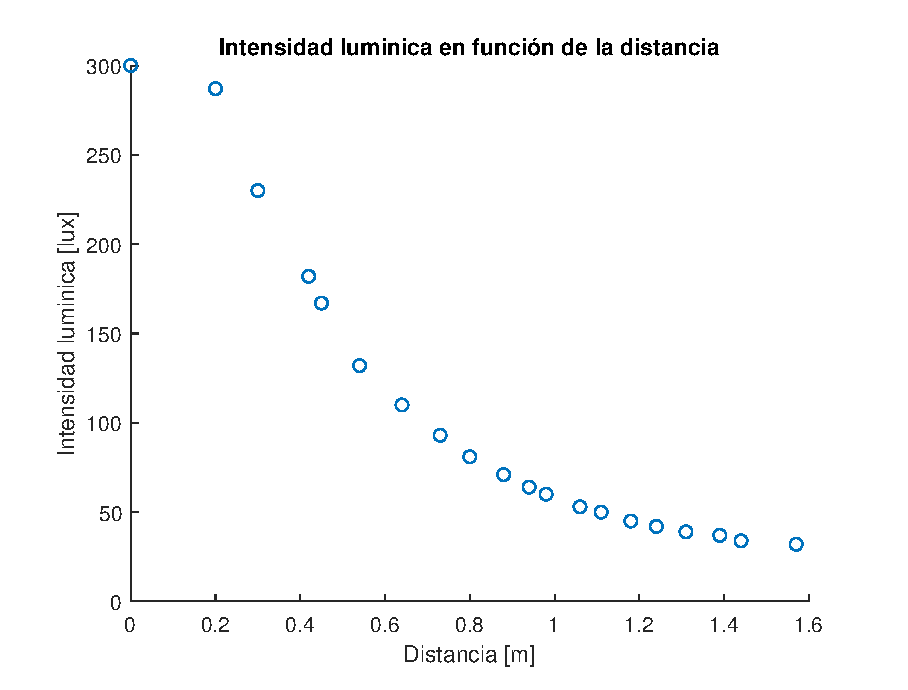
\includegraphics[scale=1.00]{resources/3.1.1.eps}
\caption{Gráfica de intensidad lumínica}
\label{practica41}
\end{figure}

La figura \ref{practica41} sugiere un modelo no lineal, así que se aplicara el
método de logaritmos.

La función tiene la forma general:

\begin{equation*}
    y = a x^b
\end{equation*}

Aplicando logaritmos a ambos lados de la ecuación, obtenemos:

\begin{equation*}
    \log y = \log a + b \log x
\end{equation*}

Haciendo los siguientes cambios de variables:

\begin{equation*}
    Y' = \log y
\end{equation*}
\begin{equation*}
    A = \log a
\end{equation*}
\begin{equation*}
    B = b
\end{equation*}
\begin{equation*}
    X' = \log x
\end{equation*}

Se obtiene:

\begin{equation*}
    Y' = A + B X'
\end{equation*}

\begin{center}
\begin{tabular}{|c|>{\centering}m{2.8cm}<{\centering}
                  |>{\centering}m{2.8cm}<{\centering}|}
\hline
$i$ & $\log(x_i)$ & $\log(I_i)$ \tabularnewline \hline
  1 & -       & -      \tabularnewline \hline
  2 & -0.6990 & 2.4579 \tabularnewline \hline
  3 & -0.5229 & 2.3617 \tabularnewline \hline
  4 & -0.3768 & 2.2601 \tabularnewline \hline
  5 & -0.3468 & 2.2227 \tabularnewline \hline
  6 & -0.2676 & 2.1206 \tabularnewline \hline
  7 & -0.1938 & 2.0414 \tabularnewline \hline
  8 & -0.1367 & 1.9685 \tabularnewline \hline
  9 & -0.0969 & 1.9085 \tabularnewline \hline
 10 & -0.0555 & 1.8513 \tabularnewline \hline
 11 & -0.0269 & 1.8062 \tabularnewline \hline
 12 & -0.0088 & 1.7782 \tabularnewline \hline
 13 &  0.0253 & 1.7243 \tabularnewline \hline
 14 &  0.0453 & 1.6990 \tabularnewline \hline
 15 &  0.0719 & 1.6532 \tabularnewline \hline
 16 &  0.0934 & 1.6232 \tabularnewline \hline
 17 &  0.1173 & 1.5911 \tabularnewline \hline
 18 &  0.1430 & 1.5682 \tabularnewline \hline
 19 &  0.1584 & 1.5315 \tabularnewline \hline
 20 &  0.1959 & 1.5051 \tabularnewline \hline
\end{tabular}
\end{center}

La gráfica de los datos con el cambio de variable logarítmica pueden verse en la
figura \ref{practica41_2}.

\begin{figure}[!h]
\centering
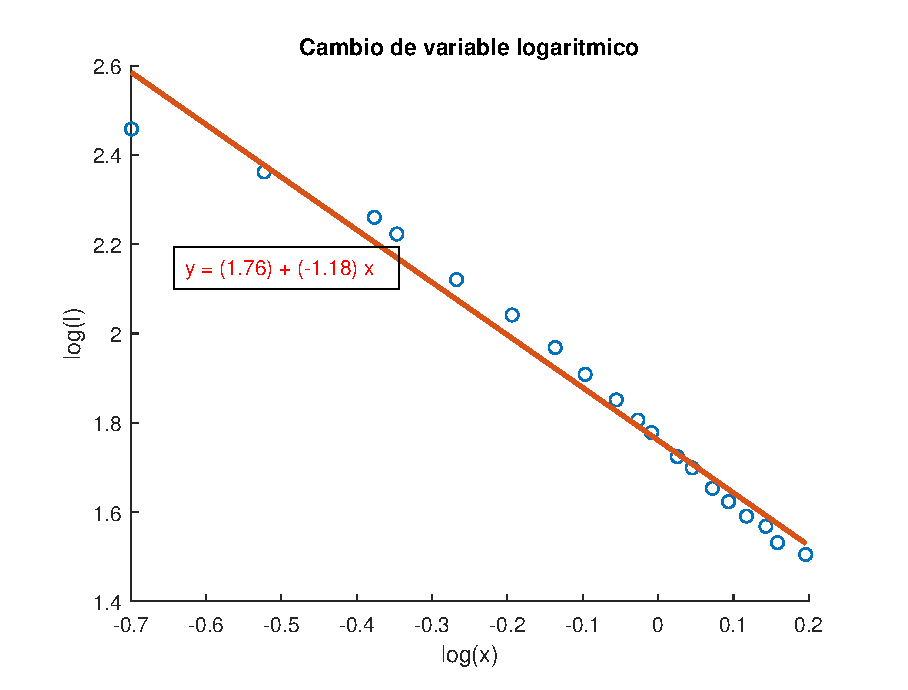
\includegraphics[scale=1.00]{resources/3.1.2.eps}
\caption{Gráfica linealizada por el método de logaritmos}
\label{practica41_2}
\end{figure}

Calculando los valores de la recta por el método de los mínimos cuadrados, se
obtiene:

\begin{equation}
    A = (1.76 \pm 0.01)[u];0.65\%
\end{equation}

\begin{equation}
    B = (-1.18 \pm 0.04)[u];3.76\%
\end{equation}

La ecuación de la recta es:

\begin{equation}
    Y = 1.76 - 1.18 x
\end{equation}

A partir de los parámetros de recta $A$ y $B$, calculamos los parámetros $a$ y
$b$, de la curva original y sus errores por el método de propagación de errores:

\begin{equation*}
    a = antilog(A) = antilog(4.05) = 57.6575
\end{equation*}
\begin{equation*}
    b = B = -1.1782
\end{equation*}
\begin{equation*}
    e_a = 10^A ln(10) e_A = 1.5250
\end{equation*}
\begin{equation*}
    e_b = e_B = 0.0443
\end{equation*}

Obteniendo finalmente los valores de la curva:

\begin{equation}
    a = (57.7 \pm 1.5)[u];2.64\%
\end{equation}

\begin{equation}
    b = (-1.18 \pm 0.04)[u];3.76\%
\end{equation}

La ecuación de la curva resultante es:

\begin{equation}
    y = 57.7 x^{-1.18}
\end{equation}

\subsubsection{Memoria de calculo}

\paragraph{Entrada del programa}
\begin{alltt}
\footnotesize
\input{resources/i3_1.csv}
\normalsize
\end{alltt}

\paragraph{Comandos del programa}
\begin{alltt}
\footnotesize
\input{resources/p4_1_2.m}
\normalsize
\end{alltt}

\paragraph{Salida del programa}
\begin{alltt}
\footnotesize
\input{resources/o4_1_2.txt}
\normalsize
\end{alltt}

\newpage
\subsection{Presión vs profundidad}
\begin{figure}[!h]
\centering
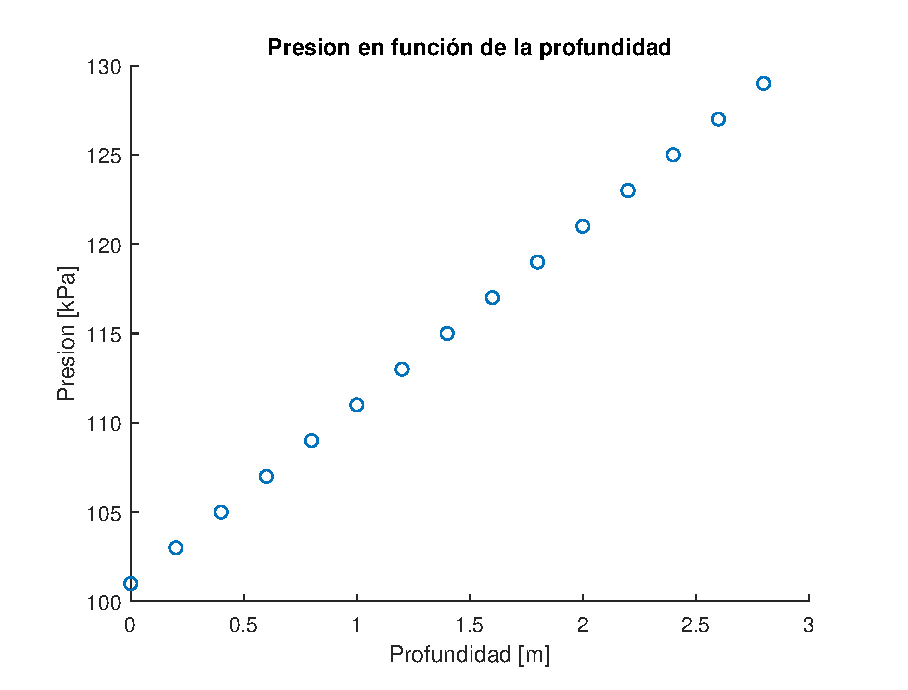
\includegraphics[scale=1.00]{resources/3.2.1.eps}
\caption{Gráfica de presión vs profundidad}
\label{practica42}
\end{figure}

La figura \ref{practica42} sugiere un modelo lineal, así que se calcularán los
valores de la recta por el método de los mínimos cuadrados.

Calculando los parámetros con \emph{Matlab} se obtienen los siguientes valores:

\begin{equation}
    A = 101 [u]
\end{equation}

\begin{equation}
    B = 10 [u]
\end{equation}

con los valores de \emph{sigma} muy próximos a cero.

La ecuación de la recta es:

\begin{equation}
    y = 101 + 10 x
\end{equation}

\begin{figure}[!h]
\centering
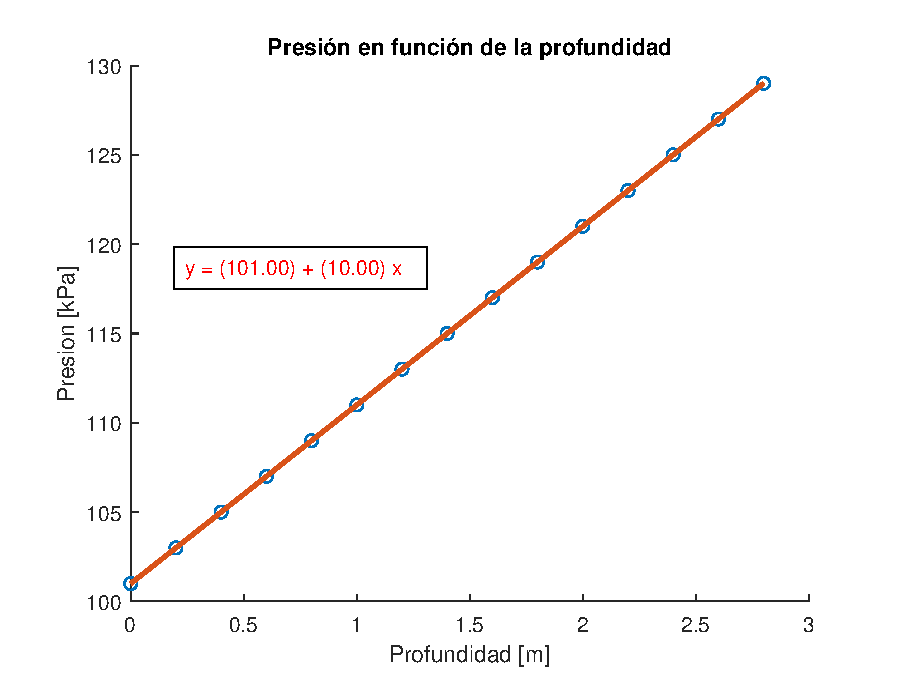
\includegraphics[scale=1.00]{resources/3.2.2.eps}
\caption{Ecuación de presión vs profundidad}
\label{practica42_2}
\end{figure}

\subsubsection{Memoria de calculo}

\paragraph{Entrada del programa}
\begin{alltt}
\footnotesize
\input{resources/i3_2.csv}
\normalsize
\end{alltt}

\paragraph{Comandos del programa}
\begin{alltt}
\footnotesize
\input{resources/p4_2_2.m}
\normalsize
\end{alltt}

\paragraph{Salida del programa}
\begin{alltt}
\footnotesize
\input{resources/o4_2_2.txt}
\normalsize
\end{alltt}

\newpage
\subsection{Resistencia vs temperatura}
\begin{figure}[!h]
\centering
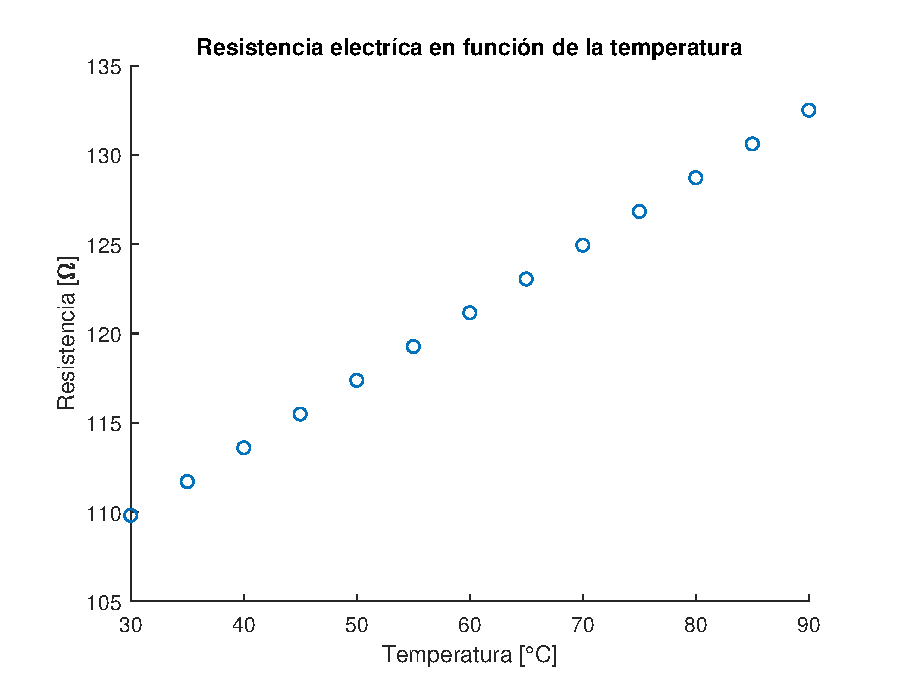
\includegraphics[scale=1.00]{resources/3.3.1.eps}
\caption{Gráfica de resistencia vs temperatura}
\label{practica43}
\end{figure}

La figura \ref{practica43} sugiere un modelo lineal, así que se calcularán los
valores de la recta por el método de los mínimos cuadrados.

Calculando los parámetros con \emph{Matlab} se obtienen los siguientes valores:

\begin{equation}
    A = 98.4800 [u]
\end{equation}

\begin{equation}
    B = 0.3780 [u]
\end{equation}

con los valores de \emph{sigma} muy próximos a cero.

La ecuación de la recta es:

\begin{equation}
    y = 98.48 + 0.38 x
\end{equation}

\begin{figure}[!h]
\centering
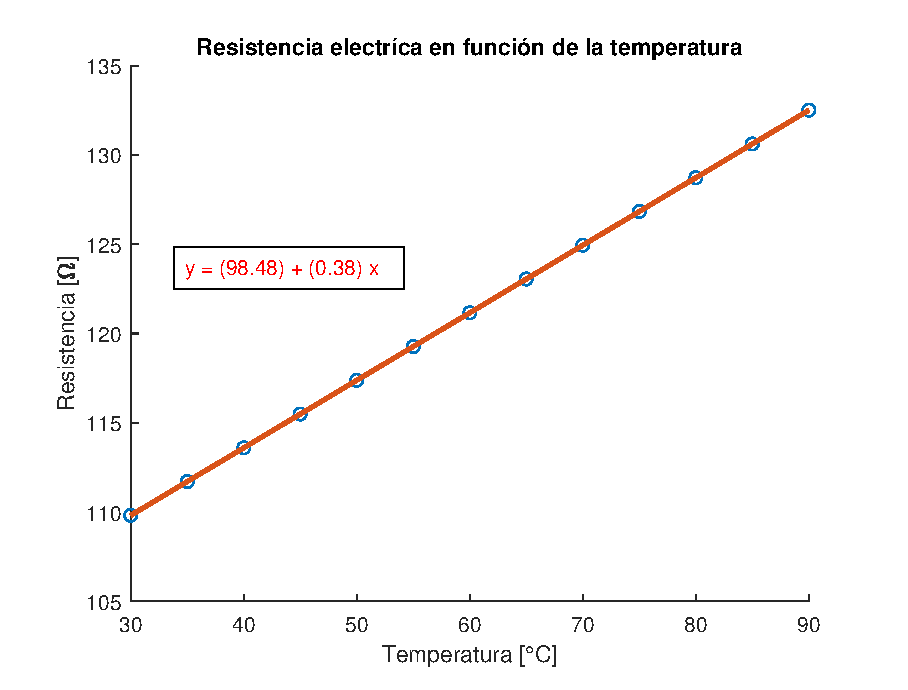
\includegraphics[scale=1.00]{resources/3.3.2.eps}
\caption{Ecuación de la resistencia vs temperatura}
\label{practica43_2}
\end{figure}

\subsubsection{Memoria de calculo}

\paragraph{Entrada del programa}
\begin{alltt}
\footnotesize
\input{resources/i3_3.csv}
\normalsize
\end{alltt}

\paragraph{Comandos del programa}
\begin{alltt}
\footnotesize
\input{resources/p4_3_2.m}
\normalsize
\end{alltt}

\paragraph{Salida del programa}
\begin{alltt}
\footnotesize
\input{resources/o4_3_2.txt}
\normalsize
\end{alltt}

\subsection{Péndulo}
\begin{figure}[!h]
\centering
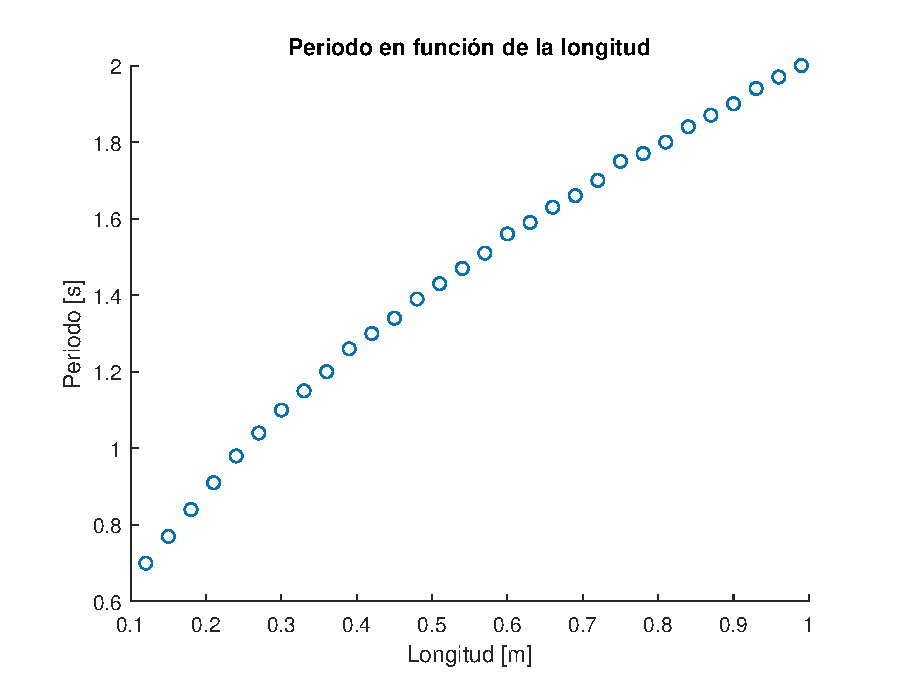
\includegraphics[scale=1.00]{resources/3.4.1.eps}
\caption{Gráfica del péndulo}
\label{practica44}
\end{figure}

La figura \ref{practica44} sugiere un modelo no lineal, así que se aplicara el
método de logaritmos.

La función tiene la forma general:

\begin{equation*}
    y = a x^b
\end{equation*}

Aplicando logaritmos a ambos lados de la ecuación, obtenemos:

\begin{equation*}
    \log y = \log a + b \log x
\end{equation*}

Haciendo los siguientes cambios de variables:

\begin{equation*}
    Y' = \log y
\end{equation*}
\begin{equation*}
    A = \log a
\end{equation*}
\begin{equation*}
    B = b
\end{equation*}
\begin{equation*}
    X' = \log x
\end{equation*}

Se obtiene:

\begin{equation*}
    Y' = A + B X'
\end{equation*}

\begin{center}
\begin{tabular}{|c|>{\centering}m{2.8cm}<{\centering}
                  |>{\centering}m{2.8cm}<{\centering}|}
\hline
$i$ & $\log(L_i)$ & $\log(T_i)$ \tabularnewline \hline
  1 &  -      &  -      \tabularnewline \hline
  2 & -0.8239 & -0.1135 \tabularnewline \hline
  3 & -0.7447 & -0.0757 \tabularnewline \hline
  4 & -0.6778 & -0.0410 \tabularnewline \hline
  5 & -0.6198 & -0.0088 \tabularnewline \hline
  6 & -0.5686 &  0.0170 \tabularnewline \hline
  7 & -0.5229 &  0.0414 \tabularnewline \hline
  8 & -0.4815 &  0.0607 \tabularnewline \hline
  9 & -0.4437 &  0.0792 \tabularnewline \hline
 10 & -0.4089 &  0.1004 \tabularnewline \hline
 11 & -0.3768 &  0.1139 \tabularnewline \hline
 12 & -0.3468 &  0.1271 \tabularnewline \hline
 13 & -0.3188 &  0.1430 \tabularnewline \hline
 14 & -0.2924 &  0.1553 \tabularnewline \hline
 15 & -0.2676 &  0.1673 \tabularnewline \hline
 16 & -0.2441 &  0.1790 \tabularnewline \hline
 17 & -0.2218 &  0.1931 \tabularnewline \hline
 18 & -0.2007 &  0.2014 \tabularnewline \hline
 19 & -0.1805 &  0.2122 \tabularnewline \hline
 20 & -0.1612 &  0.2201 \tabularnewline \hline
 21 & -0.1427 &  0.2304 \tabularnewline \hline
 22 & -0.1249 &  0.2430 \tabularnewline \hline
 23 & -0.1079 &  0.2480 \tabularnewline \hline
 24 & -0.0915 &  0.2553 \tabularnewline \hline
 25 & -0.0757 &  0.2648 \tabularnewline \hline
 26 & -0.0605 &  0.2718 \tabularnewline \hline
 27 & -0.0458 &  0.2788 \tabularnewline \hline
 28 & -0.0315 &  0.2878 \tabularnewline \hline
 29 & -0.0177 &  0.2945 \tabularnewline \hline
 30 & -0.0044 &  0.3010 \tabularnewline \hline
\end{tabular}
\end{center}

La gráfica de los datos con el cambio de variable logarítmica pueden verse en la
figura \ref{practica44_2}.

\begin{figure}[!h]
\centering
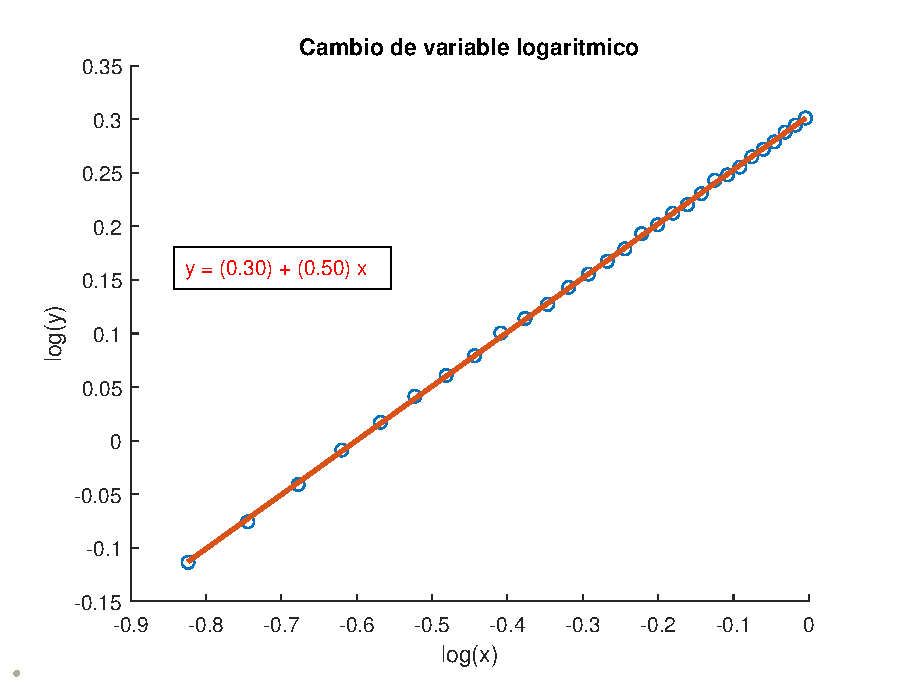
\includegraphics[scale=1.00]{resources/3.4.2.eps}
\caption{Gráfica linealizada por el método de logaritmos}
\label{practica44_2}
\end{figure}

Calculando los valores de la recta por el método de los mínimos cuadrados, se
obtiene:

\begin{equation}
    A = (0.3032 \pm 0.0004)[u];0.15\%
\end{equation}

\begin{equation}
    B = (0.505 \pm 0.001)[u];0.24\%
\end{equation}

La ecuación de la recta es:

\begin{equation}
    Y = 0.3032 - 0.505 x
\end{equation}

A partir de los parámetros de recta $A$ y $B$, calculamos los parámetros $a$ y
$b$, de la curva original y sus errores por el método de propagación de errores:

\begin{equation*}
    a = antilog(A) = antilog(4.05) = 2.0101
\end{equation*}
\begin{equation*}
    b = B = 0.5050
\end{equation*}
\begin{equation*}
    e_a = 10^A ln(10) e_A = 0.0021
\end{equation*}
\begin{equation*}
    e_b = e_B = 0.0012
\end{equation*}

Obteniendo finalmente los valores de la curva:

\begin{equation}
    a = (2.010 \pm 0.002)[u];0.10\%
\end{equation}

\begin{equation}
    b = (0.505 \pm 0.001)[u];0.24\%
\end{equation}

La ecuación de la curva resultante es:

\begin{equation}
    y = 2.01 x^{0.505}
\end{equation}

\subsubsection{Memoria de calculo}

\paragraph{Entrada del programa}
\begin{alltt}
\footnotesize
\input{resources/i3_4.csv}
\normalsize
\end{alltt}

\paragraph{Comandos del programa}
\begin{alltt}
\footnotesize
\input{resources/p4_4_2.m}
\normalsize
\end{alltt}

\paragraph{Salida del programa}
\begin{alltt}
\footnotesize
\input{resources/o4_4_2.txt}
\normalsize
\end{alltt}

\section{Conclusiones}
Se aprendió a graficar diferentes relaciones entre variables sean lineales o
no lineales, como también calcular la ecuación que rige su comportamiento.

\subsection{Resultados obtenidos}

\begin{center}
\begin{tabular}{|c|c|}
\hline
\multicolumn{2}{|c|}{\textbf{Intensidad lumínica}} \\
\multicolumn{2}{|c|}{$y = 57.7 x^{-1.18}$} \\
\hline
\multicolumn{2}{|c|}{\textbf{Presión vs profundidad}} \\
\multicolumn{2}{|c|}{$y = 101 + 10 x$} \\
\hline
\multicolumn{2}{|c|}{\textbf{Resistencia vs temperatura}} \\
\multicolumn{2}{|c|}{$y = 98.48 + 0.38 x$} \\
\hline
\multicolumn{2}{|c|}{\textbf{Péndulo}} \\
\multicolumn{2}{|c|}{$y = 2.01 x^{0.505}$} \\
\hline
\end{tabular}
\end{center}

\end{document}
